\documentclass[12pt,a4]{article}

\usepackage{graphicx}
\usepackage{amssymb}
\PassOptionsToPackage{hyphens}{url}\usepackage{hyperref}%allows urls to follow line breaks of text
\usepackage{xcolor}
\usepackage{comment}
\usepackage[german]{babel}
\usepackage{wrapfig} %allows text to wrap images



\usepackage[utf8]{inputenc}%implements vowel mutations
\raggedright %shifts text to the left page border


%\begin{comment}

%sets colors for links
\hypersetup{
	colorlinks=false,
	urlbordercolor=red,
	%urlcolor=red,
	%linkcolor=red,
	%filecolor=red,      
	%urlcolor=red,
	pdftitle={Programmierung von Systemen},
	%bookmarks=true,
	%pdfpagemode=FullScreen,
}
%\end{comment}
%the figure element allows you to insert a logo on the title page
\title{
	\begin{figure}
		\centering
		
\includegraphics[height=1.5cm]{logo.png}
	\end{figure}
Programmierung von Systemen 
}

\author{Erik Neller | Dozent: Matthias Tichy}
%\date{18.08.2020}

\begin{document}
	
	\maketitle
	\thispagestyle{empty} %removes page number from title
	\newpage
	
	\tableofcontents
	\newpage
	

	\section{UML-Klassendiagramme}
	\subsection{Klassen und Schnittstellen}
	Methoden und Attribute werden wie in Java in der Form \texttt{\$TYP \$NAME} angegeben, ist die Methode vom Typ \texttt{void} entfällt der Rückgabetyp.
	\begin{itemize}
		\item \texttt{private} wird durch ''-'' symbolisiert
		\item \texttt{package} wird durch ''{\raise.17ex\hbox{$\scriptstyle\sim$}}'' symbolisiert
		\item \texttt{protected} wird durch ''\#'' symbolisiert
		\item \texttt{public} wird durch ''+'' symbolisiert
		\item \texttt{static}  wird \underline{unterstrichen}
	\end{itemize}
	\texttt{\{readonly\}} ist ein UML Attribut das für Konstanten verwendet wird. 
	\newline\newline
	
	Der Block einer Klasse / eines Interfaces besteht aus drei Feldern: 
	\begin{enumerate}
		\item Name mit Modifikatoren
		\item Attribute (Variablen)
		\item Methoden
	\end{enumerate}
	 Modifikatoren für die Klasse können sein: \texttt{\flqq interface\frqq} oder \texttt{\{abstract\}} bzw. der Name in \textit{kursiv}.
	 
	 Die Multiplizität wird genutzt um Listen und Mengen von Objekten anzugeben, aber auch in Relationen zwischen Klassen:
	 \begin{center}
	 	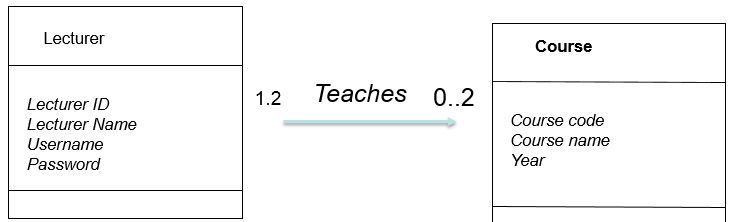
\includegraphics[width=0.5\linewidth]{images/multiplicity}
	 \end{center}
	 \begin{enumerate}
	 	\item Typ
	 	\item Größe begrenzt \{1..x\} oder unendlich [*]
	 	\item Attribute wie \{order\} und \{unique\}
	 \end{enumerate}

	 \subsection{Relationen}

 	\texttt{extends} oder \texttt{implements} wird dargestellt durch einen nicht ausgefüllten Pfeil, wobei die Linie bei gleichen Typen (Interface erbt von Interface, Klasse von Klasse) durchgezogen ist, wenn eine Klasse ein Interface implementiert, gestrichelt.
 	
 	\begin{center}
 		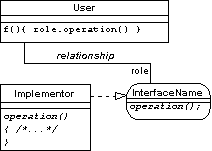
\includegraphics[width=0.5\linewidth]{images/interface1}
 	\end{center}

		
	 
	 \begin{itemize}
	 	\item Abhängigkeit (Dependency): User nutzt Ressource, aber die Ressource ist nicht Teil der User Klasse. Wird die Ressource modifiziert, muss auch der User modifiziert werden. 
	 		\begin{center}
	 		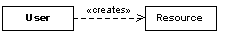
\includegraphics[width=0.5\linewidth]{images/dependency}
	 		\end{center}
 		
 		\item Aggregation: ''ist Teil von'', wird symbolisiert durch einen Pfeil mit leerer Raute
	 	\begin{center}
	 		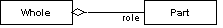
\includegraphics[width=0.5\linewidth]{images/aggregation}
	 	\end{center}
	 	
	 	\item Komposition ''besteht aus'', wird symbolisiert durch einen Pfeil mit ausgefüllter Raute
	 	\begin{center}
	 		
\includegraphics[width=0.5\linewidth]{images/composition}
	 	\end{center}
 	
 		\item Assoziation: Die Klassen sind auf eine beliebige Weise verbunden, nutzen Methoden der anderen aber nicht auf die oben genannten Weisen
 		\begin{center}
 			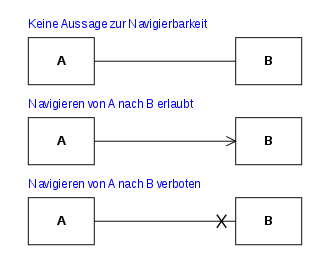
\includegraphics[width=0.4\linewidth]{images/association}
 		\end{center}
	 \end{itemize}
	
	Kommentare werden mit einer gestrichelten Linie mit dem eigentlichen Objekt verbunden.
	
	
	\section{Version Control Systems}

	\subsection{Grundlegende Funktionen}
		Version Control Systems (VCS) erlauben die Verwaltung von mehreren Teilen und Versionen eines Projekts und damit die Zusammenarbeit von mehreren Teilnehmern.
	\begin{itemize}
		\item Rechteverwaltung (z.B. Entwickler von Front-und Backend, Projektmanagement)
		\item Archivierung in verschiedenen Versionen (einfach anhand der gemachten Änderung, anstatt vollständige Backups zu machen)
		\item Speicherung von Metadaten: Historie von Änderungen mit Datum, Autor, etc.
		\item Backup zur Wiederherstellung lokal gelöschter Daten oder versehentlicher Änderungen
		\item Zentralisierung auf Server
		
	\end{itemize}
	\subsection{Git}
	Das Git System besteht aus vier Teilen, von denen drei durch Git selbst implementiert werden. Jede Änderung durchläuft sie in dieser Reihenfolge: 
	\begin{enumerate}
		\item Der eigentlichen Arbeitsplatz / \textit{Workspace} in dem Änderungen an Dateien vorgenommen werden
		\item Die \textit{staging area}, in der \textit{commits} aus einzelnen Änderungen an Dateien feingranular (bis zu einzelnen Zeilen) zusammengesetzt werden
		\item Das \textit{lokalen Repository}
		\item Das \textit{remote Repository} auf einem Server, beispielsweise GitHub oder GitLab
	\end{enumerate}
	Auf den einzelnen Bereichen existieren verschiedene Befehle. Für die staging area:
	\begin{itemize}
		\item \texttt{git init} erstellt ein neues Git-Repository im aktuellen Verzeichnis
		\item \texttt{git add} um Dateien der staging area hinzuzufügen
		\item In einer \texttt{.gitignore} Datei können Regeln für Dateien angegeben werden, die generell nicht mit in die staging area aufgenommen werden sollen
		\item \texttt{git status} um aktuell geänderte und getrackte Dateien zu sehen
		\item \texttt{git rm --cached} um Dateien aus der staging area zu entfernen
		
	\end{itemize}
	%\newline
	Für das lokale Repository:
	\begin{itemize}
		\item \texttt{git commit -m \$MESSAGE} um den Inhalt der staging area in das lokale Repository hinzuzufügen
		\item \texttt{git checkout \$COMMIT-HASH} erlaubt das Wiederherstellen vorheriger Zustände von commits
		\item \texttt{git reset --soft HEAD{\raise.17ex\hbox{$\scriptstyle\sim$}}x} erlaubt das Rückgängigmachen von x commits
		\item \texttt{git log} zeigt den Verlauf von commits an
		\item \texttt{git remote add \$NAME \$ADDRESS} verknüpft das lokale Repository mit einem remote Repository
	\end{itemize}

	Und für das remote Repository:
	\begin{itemize}
		\item \texttt{git push \$REPOSITORY \$BRANCH} um den lokalen commit auf den Server zu legen
		\item \texttt{git pull} um das lokale Repository mit den Änderungen aus dem remote Repository zu aktualisieren
		\item \texttt{git clone \$REPOSITORY} um das ganze Repository lokal zu speichern
	\end{itemize}


	
	Für verschiedene Themengebiete / Zuständigkeitsbereiche existiert das Konzept von Branches(Verzweigungen), die mit \texttt{git branch \$NAME} erstellt werden können, um anschließend mit \texttt{git checkout \$NAME} in den Branch zu wechseln, oder in Kurzform: \texttt{git checkout -b \$NAME}. Mit \texttt{git merge \$NAME} kann dann ein Branch in den jeweils Aktuellen integriert, oder mit \texttt{git branch -d \$NAME} gelöscht werden. Ist keine automatische Vereinigung der Branches möglich, müssen die angezeigten Dateien manuell geändert und anschließend mit \texttt{git add \$FILE} Alternativ kann der Branch in das Repository aufgenommen werden: \texttt{git push \$REMOTE \$BRANCH}.
	
	
	


	\section{Objektorientierung}
	\subsection{Interfaces}
	Analog zur abstrakten Klasse erlaubt ein Interface keine Instanziierung. Es enthält keine tatsächliche Implementierung, sondern nur Methodenrümpfe und evtl. Konstanten und muss dementsprechend in jeder Klasse mit dem Schlüsselwort \texttt{implements} implementiert werden. Im Gegensatz zu abstrakten Klassen können mehrere Interfaces von einer Klasse implementiert werden.
	
	\subsection{Sichtbarkeit}
	
	\begin{center}
		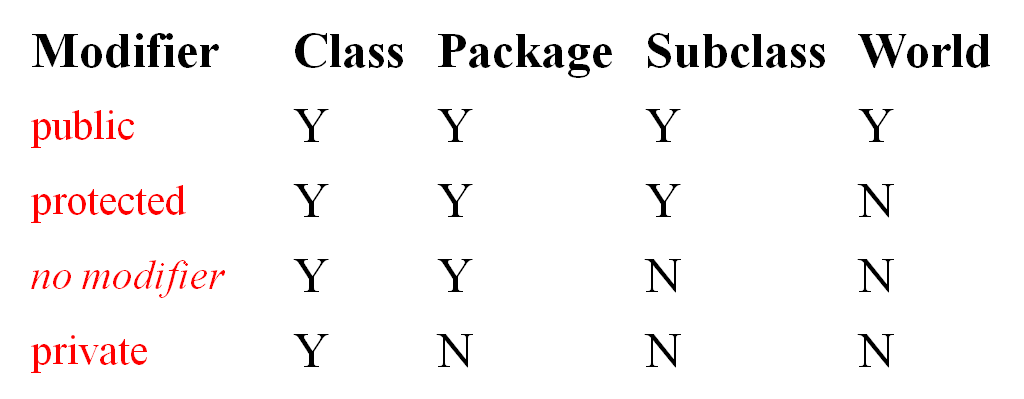
\includegraphics[width=0.7\linewidth]{images/modifiers}
	\end{center}
	
	
	\subsection{Annotations}
	Verschiedene Standardannotationen, eigene definierbar. Durch Reflection zur Laufzeit auslesbar.
	\begin{itemize}
		\item \texttt{@Override} gibt an dass hier ein Element überschrieben werden soll
		\item \texttt{@Deprecated} gibt eine Warnung aus dass Element veraltet ist
		\item \texttt{@SuppressWarnings()} unterdrückt die angegebene Warnung
		\item \texttt{@Documented} nimmt nachfolgende Annotationen in die JavaDoc mit auf
	\end{itemize}
	JavaDoc:
	\begin{itemize}
		\item \texttt{@author}
		\item \texttt{@version}
		\item \texttt{@param} zur Beschreibung von Methodenparametern
		\item \texttt{@return} beschreibt den Rückgabewert
		\item \texttt{@exception}, \texttt{@throws} Beschreibt Fehlermeldungen, die diese Methode produzieren kann
		\item \texttt{@link} Verknüpfung zu anderem Symbol
	\end{itemize}
	
	\subsection{Enumerations}
	Mit einem \texttt{enum} kann eine Menge von Konstanten definiert werden, entweder auf Klassenlevel oder innerhalb einer Klasse. Sie sind auch selbst eine Klasse, deren Attribute \texttt{public static final} definiert sind. Methoden: 
	\begin{itemize}
		\item \texttt{int ordinal()} gibt die Position in der Liste des Enums zurück
		\item \texttt{String name()} gibt den Namen der Konstanten zurück
		\item \texttt{int valueOf} gibt den zugeordneten Wert der Variablen zurück 
	\end{itemize}
	
	\section{Collections}
	\subsection{Datenstrukturen}
	\subsubsection{Array}
	Statische Größe, wird mit Länge und Datentyp gespeichert, zB int[5]. Objekt x erhalten: array[x]. Länge: array.length
	\subsubsection{ArrayList}
	Klasse die zur Speicherung Arrays verwendet, diese aber ersetzt wenn die Methoden \texttt{add()} oder \texttt{remove()} aufgerufen werden. Mit \texttt{toArray()} kann der Array erhalten werden, mit \texttt{size()} die Größe, da diese dynamisch ist. Objekt erhalten: arraylist.get(x).
	\subsubsection{Linked List}
	Jedes Listenelement enthält einen Zeiger auf das nächste Element, bei dem letzten Element ist der Zeiger \texttt{NULL}.
	\subsubsection{Double Linked List}
	Wie linked list, nur dass jedes Element zusätzlich einen Zeiger auf das vorherige Element enthält (beim ersten Element \texttt{NULL}).
	\subsubsection{Sorted Tree}
	Setzt die Sortierbarkeit der Objekte voraus: Objekte mit kleinerem Wert sind links des Vaterknotens, mit größerem rechts. Beim Einfügen / Entfernen reorganisieren: rot-schwarz Bäume, B Baum, B+Baum
	\begin{center}
		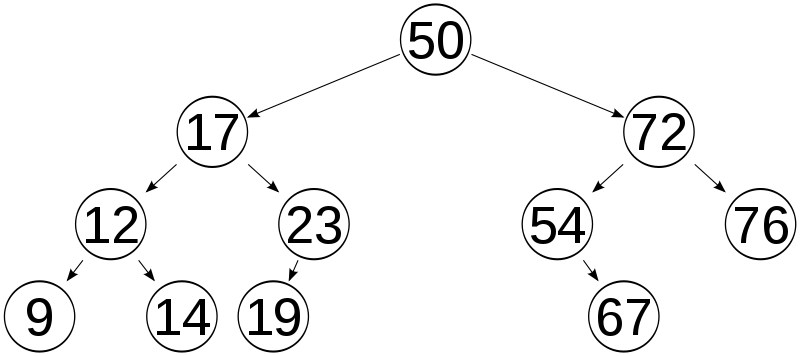
\includegraphics[width=0.5\linewidth]{images/sortedtree}
	\end{center}
	\subsubsection{HashTable}
	Objekte werden gehasht, also ein Wert aus ihnen berechnet, anhand dessen sie in in eine Tabelle eingeordnet werden.
	\subsubsection{Map}
	Speichert nicht einzelne Werte, sondern Tupel aus (Key, Value), nutzt dann zB eine Liste aus Tupeln oder eine Hashtabelle anhand der Keys.
	
	\subsection{Collections API}
	Stellt effiziente Datenstrukturen für viele Anwendunge bereit, sodass Datenstrukturen und Algorithmen nicht selbst implementiert werden müssen.
	Das Collection Interface selbst enthält Methoden wie add(), size(), contains(), remove()
	\begin{itemize}
	
	\item List ist eine geordnete Collection: add(e), add(index, e), indexOf(e), contains(e) 
	\item Set ist eine Collection ohne Duplikate(inklusive \texttt{NULL}): add(), contains()
	\end{itemize}
	\subsection{Queue}
	Warteschlange als Datenstruktur bei der Elemente am einen Ende angehängt und am anderen Ende gelesen werden. Dementsprechend existieren die folgenden Methoden, die eine Exception verursachen bei Fehlern:
	
	\begin{itemize}
		\item add(e) fügt ein Element hinten an der Queue an, falls max. Größe erreicht Exception
		\item remove() nimmt das vorderste Element der Queue und gibt es zurück, gleichzeitig wird es aus der Queue entfernt (Exception falls Queue leer)
		\item element() gibt das erste Element aus der Queue zurück aber löscht es nicht (ebenfalls Exception falls leer)
	\end{itemize}

	Alternativ existieren die Methoden mit speziellen Rückgabewerten anstelle von Exceptions:
	\begin{itemize}
		\item offer(e) gibt true/false zurück ob Element hinzugefügt wurde
		\item poll() gibt Element oder \texttt{NULL} zurück
		\item peek() gibt Element oder \texttt{NULL} zurück
	\end{itemize}

	\subsection{Deque}
	Ist die Erweiterung einer Queue mit den gleichen Operationen an beiden Enden der Datenstruktur, analog zu einem Kartendeck.
	
	\subsubsection{Exception und special Element}
	
\begin{tabular}{|c|c|c|c|c|}
	\hline 
	&\multicolumn{2}{|c|}{\textbf{throw Exception}}&\multicolumn{2}{|c|}{\textbf{special Element}} \\
	\hline 
	&\textit{first}&\textit{last}&\textit{first}&\textit{last}  \\ 
	\hline 
	\textbf{einfügen}&addFirst()&addLast()&offerFirst()&offerLast()\\ 
	\hline 
	\textbf{löschen}&  removeFirst()&removeLast()&pollFirst()&pollLast()\\ 
	\hline 
	\textbf{lesen}(behalten)&getFirst()&getLast()&peekFirst()&peekLast()\\ 
	\hline 
\end{tabular} 

	\subsubsection{Blocking Deque}
	Die dritte Möglichkeit ist den Thread zu blockieren wenn die Operation nicht möglich ist. Davon existieren zwei Varianten: mit maximaler Blockierungszeit (Timeout) und ohne. Dieses blocking deque implementiert sowohl die blocking Queue (welche queue und blocking implementiert) als auch das Deque.
	\begin{center}
	\begin{tabular}{|c|c|c|}
		\hline 
		&\textbf{block}&\textbf{timeout}\\ 
		\hline 
		\textbf{einfügen}&putFirst()&offerFirst(e,time,unit)\\ 
		\hline 
		\textbf{löschen}&takeFirst()&pollFirst(e,time,unit)\\ 
		\hline 
		\textbf{lesen}(behalten)&-&-  \\ 
		\hline 
	\end{tabular} 
	\end{center}
	\subsection{Generics}
	Collections können \textit{generisch} verwendet werden, indem bei der Initialisierung eine Klasse angegeben wird, deren Instanzen in der Collection enthalten sein werden. Bei allen anderen Klassen / Datentypen wird der Compiler hier direkt eine Fehlermeldung liefern, was der Alternative, potenzielle Fehler während der Laufzeit, vorzuziehen ist.
	\subsection{Streams}
	Streams aus \texttt{java.util.stram.Stream<T>} stellen Ströme von Referenzen dar, die es erlauben, verkettete Operationen auf diesem Datenstrom nacheinander oder parallel auszuführen. Bestimmte Methoden erlauben die Verwendung von Prädikaten und klassischen mathematischen Funktionen. Wo vorher eine for-Schleife mit Zählvariable notwendig war um die Anzahl von bestimmten Elementen in einem Array zu erhalten, kann man damit schreiben: \texttt{anzahl = Arrays.stream(myArray).filter(x -> x.equals("String")).count();}
	
	\section{IO Streams}
	
	
	
	
	
	
	
	
	
\end{document}